\section{Toric Variety of Projective Spaces}
\label{sec:toric-variety-of-projective-spaces}
    We see in Section \ref{sec:tropical-arithmetic-valuations-tropical-plane-curves} that tropical varieties induce interesting combinatorial objects and polyhedral complexes give us tools for viewing old problems in new ways.
    We now introduce \textbf{polytopes}
    more formally and actually connect fans and their associated toric varieties with polytopes.
    In this section we follow the treatment and examples of \citet{Fulton1993} and \citet{Ranganathan2012}
    
    Roughly put, given a polytope, 
    we can define a fan whose rays are normal to the facets of the polytope that is determined by the toric variety associated with the fan.
    Here we don't give explicit constructions of these polytope but only show these polytopes and their associated projective spaces, to help the readers gain some geometric intuition.

        The polytope of $\P^3$, 
        which we have shown is a toric variety, 
        is the tetrahedron. 
        
        \begin{figure}
        \label{fig:tetrahedron}
        \begin{center}
        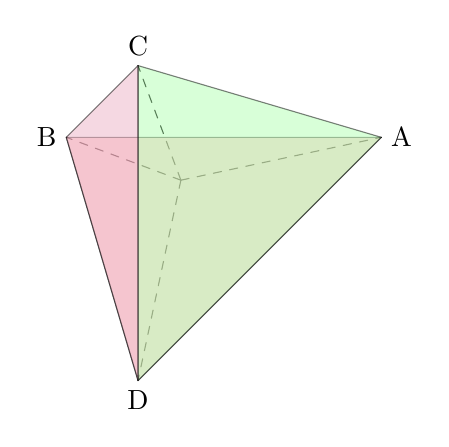
\begin{tikzpicture}[line join = round, line cap = round]
        \pgfmathsetmacro{\factor}{1/sqrt(2)};
        \coordinate [label=right:A] (A) at (2,0,-2*\factor);
        \coordinate [label=left:B] (B) at (-2,0,-2*\factor);
        \coordinate [label=above:C] (C) at (0,2,2*\factor);
        \coordinate [label=below:D] (D) at (0,-2,2*\factor);

        \foreach \i in {A,B,C,D}
        \draw[dashed] (0,0)--(\i);
        \draw[-, fill=red!30, opacity=.5] (A)--(D)--(B)--cycle;
        \draw[-, fill=green!30, opacity=.5] (A) --(D)--(C)--cycle;
        \draw[-, fill=purple!30, opacity=.5] (B)--(D)--(C)--cycle;
        \end{tikzpicture}
        \end{center}
        \caption{A tetrahedron, the polytope of $\P^3$}
        \end{figure}
        
        \begin{figure}
        \label{fig:fan-p2}
	    \begin{center}
	    \begin{tikzpicture}[axis/.style={thin, ->, >=stealth'}]
	    % Draw coordinates
		\draw[axis] (0, 0) -- (1, 0) node[right]{$v_1$};
		\draw[axis] (0, 0) -- (0, 1)
		node[above]{$v_2$};
		\draw[axis] (0, 0) -- (-1, -1) node[below]{$v_3$};
	    \end{tikzpicture}
	    \end{center}
	    \caption{The fan of $\P^2$.}
        \end{figure}
        
        \begin{figure}
        \begin{center}
        \begin{tikzpicture}
        \label{fig:polytope-p2}
        \draw (-2,0) node[anchor=north]{$A$}
        -- (2,0) node[anchor=north]{$C$}
        -- (0,4) node[anchor=south]{$B$}
        -- cycle;
        \end{tikzpicture}
        \end{center}
        \caption{The polytope of $\P^2$}
        \end{figure}
        
        \begin{figure}
        \label{fig:fan-p1-p1}
	    \begin{center}
	    \begin{tikzpicture}[axis/.style={thin, ->, >=stealth'}]
	    % Draw coordinates
		\draw[axis] (0, 0) -- (1, 0) node[right]{$v_1$};
		\draw[axis] (0, 0) -- (0, 1)
		node[above]{$v_2$};
		\draw[axis] (0, 0) -- (-1, 0) node[below]{$v_3$};
		\draw[axis] (0, 0) -- (0, -1) node[below]{$v_4$};
	    \end{tikzpicture}
	    \end{center}
	    \caption{The fan of $\P^1 \times \P^1$.}
        \end{figure}
        
        \begin{figure}
        \label{fig:polytope-p1-p1}
        \begin{center}
        \begin{tikzpicture}
        \draw (1,1) node[anchor=south]{$A$}
        -- (-1,1) node[anchor=south]{$B$}
        -- (-1,-1) node[anchor=north]{$C$}
        -- (1,-1) node[anchor=north]{$D$}
        -- cycle;
        \end{tikzpicture}
        \end{center}
        \caption{The polytope of $\P^1 \times \P^1$}
        \end{figure}
    
        \begin{figure}
        \label{fig:polytope-p1-p1-p1}
        \begin{center}
        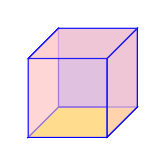
\begin{tikzpicture}
        \coordinate (O) at (0,0,0);
        \coordinate (A) at (0,\Width,0);
        \coordinate (B) at (0,\Width,\Height);
        \coordinate (C) at (0,0,\Height);
        \coordinate (D) at (\Depth,0,0);
        \coordinate (E) at (\Depth,\Width,0);
        \coordinate (F) at (\Depth,\Width,\Height);
        \coordinate (G) at (\Depth,0,\Height);

        \draw[blue,fill=yellow!80] (O) -- (C) -- (G) -- (D) -- cycle;% Bottom Face
        \draw[blue,fill=blue!30] (O) -- (A) -- (E) -- (D) -- cycle;% Back Face
        \draw[blue,fill=red!10] (O) -- (A) -- (B) -- (C) -- cycle;% Left Face
        \draw[blue,fill=red!20,opacity=0.8] (D) -- (E) -- (F) -- (G) -- cycle;% Right Face
        \draw[blue,fill=red!20,opacity=0.6] (C) -- (B) -- (F) -- (G) -- cycle;% Front Face
        \draw[blue,fill=red!20,opacity=0.8] (A) -- (B) -- (F) -- (E) -- cycle;% Top Face
        \end{tikzpicture}
        \end{center}
        \caption{The polytope of $\P^1 \times \P^1 \times \P^1$}
        \end{figure}
    